\documentclass[12pt]{article}

\usepackage[hidelinks]{hyperref}
\usepackage{float}
\usepackage{tabularx}
\usepackage{longtable}
\usepackage{circuitikz}
% (opcional, si quieres \si{\ohm}):
% \usepackage{siunitx}
\usepackage{tabularx} % en el preámbulo
\usepackage[utf8]{inputenc}
\usepackage[spanish, mexico]{babel}
\usepackage{graphicx}
\usepackage[letterpaper, margin=2.5cm]{geometry}
\usepackage{fancyhdr}
\usepackage[justification=centering]{caption}
\usepackage{float}
\usepackage{titlesec}
\usepackage{multirow}
\usepackage{lmodern}
\usepackage{amsmath}
\usepackage{titling}
\usepackage{enumitem}
\usepackage{listings}
\usepackage{xcolor}
\usepackage{svg}
\usepackage{rotating}
\usepackage{tocloft}
\usepackage{multicol}
\usepackage{steinmetz}
\usepackage{amssymb}
\usepackage{tikz}
\usepackage{multirow}
\usepackage[siunitx]{circuitikz}
\usepackage{amsmath} 
\usepackage{booktabs} 



\usepackage{siunitx}
\usepackage{siunitx,makecell,multirow,hhline}
\sisetup{output-decimal-marker = {,}, detect-all = true}
\newcommand{\thickrule}{\Xhline{1.1pt}}   % borde superior/inferior más grueso
\setlength{\arrayrulewidth}{0.6pt}
\renewcommand\arraystretch{1.2}
\usepackage{siunitx,booktabs,makecell,xcolor,colortbl}
\sisetup{output-decimal-marker = {,}, detect-all = true} % coma decimal
% sombreado alternado opcional (comenta si no lo quieres)
\rowcolors{2}{gray!6}{white}

\usetikzlibrary{angles, arrows.meta, quotes}
\usepackage{siunitx}
\DeclareSIUnit\voltampere{VA}   % apparent power
\DeclareSIUnit\var{VAR}   

\usepackage{graphicx}
\usepackage{subcaption}
\graphicspath{{Recursos/}} % carpeta donde están los PDF


\lstdefinelanguage{Matlab}{
  keywords={break,case,catch,continue,else,elseif,end,for,function,
      global,if,otherwise,persistent,return,switch,try,while},
  keywordstyle=\color{blue}\bfseries,
  identifierstyle=\color{black},
  commentstyle=\color{gray}\ttfamily,
  stringstyle=\color{red},
  sensitive=true
}

\lstset{
  language=Matlab,
  frame=single,
  basicstyle=\ttfamily\footnotesize,
  keywordstyle=\color{blue},
  commentstyle=\color{gray},
  stringstyle=\color{red},
  numbers=left,
  numberstyle=\tiny\color{gray},
  numbersep=5pt,
  showstringspaces=false,
  breaklines=true,
  captionpos=b
}

\hypersetup{
  colorlinks=true,
  linkcolor=blue,
  citecolor=green,
  urlcolor=cyan
}

% Márgenes y espacio
\geometry{top=2.5cm, bottom=2.5cm, left=3cm, right=3cm}
\setlength{\parskip}{0.8em}
\setlength{\parindent}{0pt}

% Encabezado y pie de página
\pagestyle{fancy}
\fancyhf{}
\lhead{ELI-214 Metrología Eléctrica}
\rfoot{Experiencia 3}
\lfoot{USM 2025-2}
\rhead{\thepage}
\renewcommand{\headrulewidth}{0.4pt}
\renewcommand{\footrulewidth}{0.4pt}
\renewcommand{\arraystretch}{1.5}


\begin{document}

% -------------------- PORTADA --------------------
\begin{titlepage}
    \centering
    
\includegraphics[width=0.85\textwidth]{logoDepEliUSM.png}
    


    \vspace{2.4cm}
    \Large \textbf{[ELI214] - Metrología Eléctrica}\\
    
    \vspace{1.2cm}
    \rule{\textwidth}{0.4pt}
    
    \vspace{0.5cm}
    \Huge \textbf{Experiencia N° 3}
    
    \vspace{0.3cm}
    \large  “Parte 2: Amperímetro de bobina móvil”
    
    \vspace{0.5cm}
    \rule{\textwidth}{0.4pt}
    
    \vfill
    \begin{flushleft}
        \textbf{Autores:} \\
        Cristóbal Daniel Jara Poblete\\
        Jean Franco Gatica Turra \\[1em]

        \textbf{Grupo 4}\\[1em]
        
        \textbf{Profesor:} Juan Guillermo Navarrete \'Alvarez\\[1em]
        
        \textbf{Fecha:} 15 de octubre de 2025
    \end{flushleft}
\end{titlepage}

\newpage

\begin{small}  % o \footnotesize o \scriptsize
\tableofcontents
\end{small}
\newpage

\section{Resumen Ejecutivo}
Diseño y prueba de un amperímetro analógico de tres rangos (10, 50 y 100 mA) construido a partir de un galvanómetro. Se cumplieron los objetivos de calibrar el instrumento y verificar sus principios de funcionamiento. La calibración se fijó en el rango de 100 mA, lo que permitió medir el error sistemático inducido en los rangos inferiores, resultando en desviaciones significativas de $\approx 14\%$ en los fondos de escala de 10 mA y 50 mA. Se comprobó exitosamente la linealidad del instrumento, con un $R^2 > 0.996$ en todos los rangos, validando el diseño teórico. Finalmente, se cuantificó el efecto de carga, demostrando que la resistencia interna del amperímetro perturba la medición (ej. alterando la corriente en $5.74\%$ en el rango de 50 mA versus $2.97\%$ en el de 100 mA), confirmando que el instrumento afecta al sistema original y que su precisión depende críticamente de una calibración adecuada para cada rango o encontrar correctamente los errores admisibles.

\section{Introducción}
La metrología es una disciplina fundamental en la ingeniería, considerada el arte de medir. Su objetivo principal es garantizar que las mediciones sean precisas y confiables, permitiendo que los resultados obtenidos sean comparables y verificables. En este contexto, el diseño de instrumentos de medición precisos y fiables es de crucial importancia, y estos deben ser contrastados con otros instrumentos de mayor precisión para asegurar la validez de las mediciones.

Es igualmente importante comprender el impacto que tiene la medición sobre el propio sistema. Al incorporar un instrumento de medición a un circuito o sistema, se introduce una perturbación inevitable, ya que el propio dispositivo de medición altera las condiciones del sistema. Esto implica que nunca será posible conocer los valores exactos de las magnitudes que se miden. Sin embargo, mediante un análisis adecuado, es posible determinar una cota de error que nos permita aproximarnos a los valores reales, garantizando la confiabilidad de los resultados.

En la primera parte de esta experiencia de laboratorio, se exploró el funcionamiento del galvanómetro y su comportamiento como filtro pasa bajos. También se realizó el diseño y prueba de un voltímetro analógico, utilizando este mismo galvanómetro. Como continuación natural de este trabajo, en esta segunda parte se procederá a la construcción de un amperímetro analógico, también basado en el galvanómetro de bobina móvil.

Para la realización de este amperímetro, se llevarán a cabo cálculos teóricos, simulaciones, y finalmente el diseño físico del instrumento. Este se calibrará adecuadamente y se pondrá a prueba en distintos rangos de medición, contrastando sus resultados con los obtenidos por instrumentos de mayor precisión para verificar su exactitud.

\subsection{Objetivos}
\subsubsection*{Objetivos Generales}
\begin{itemize}
    \item Diseñar un amperímetro analógico de tres rangos a partir de un galvanómetro de bobina móvil.
    \item Comprender el principio de funcionamiento de un amperímetro analógico y las protecciones que debe incluir. 
\end{itemize}

\subsubsection*{Objetivos Específicos}
\begin{itemize}
    \item Calibrar un amperímetro para el máximo rango de medición
    \item Medir el error inducido en mediciones de un rango inferior 
    \item Comprobar la linealidad de un instrumento analógico compuesto por elementos pasivos.
\end{itemize}

\section{Marco Teórico}

\subsection{Principio de funcionamiento de Amperímetro}
Un amperímetro de bobina móvil se construye utilizando un galvanómetro, un dispositivo muy sensible a pequeñas magnitudes de corriente. El principio básico de este amperímetro es medir la corriente eléctrica que fluye a través de un circuito; sin embargo, dado que el galvanómetro está diseñado para medir corrientes muy bajas, es necesario adaptarlo para poder medir rangos más grandes de corriente sin dañar el dispositivo.

Para lograr esto, se utiliza un divisor de corriente mediante una resistencia shunt en paralelo con el galvanómetro. Esta resistencia, que generalmente tiene un valor muy bajo comparada a la resistencia interna del galvanómetro, permite que una porción de la corriente fluya a través de ella, protegiendo el galvanómetro. De este modo, solo una fracción de la corriente total pasa por el galvanómetro, permitiendo que se utilice para medir corrientes mucho mayores sin que el dispositivo se dañe.

\subsubsection{Cálculo de Resistencias Shunt}
La resistencia shunt $R_s$ se calcula teniendo en cuenta la corriente máxima que se desea medir y la resistencia $R_g$ interna del galvanómetro. El objetivo es asegurar que cuando se mida la corriente máxima, la corriente que pase por el galvanómetro no exceda su corriente máxima admisible $I_{g\ max}$, la cual es determinada por la sensibilidad $s$ del galvanómetro como $I_{g\ max} = 1/s$.

Una vez fijada la corriente máxima para el galvanómetro, la resistencia shunt necesaria para cada rango se determina a partir de la siguiente fórmula:

\begin{equation}
    R_{sh} = R_g \cdot \frac{I_m}{I_{\text{rango}} - I_m}
    \label{eq:Rsh}
\end{equation}

Donde $I_{rango}$ es la corriente máxima que se desea medir en un rango específico del amperímetro.

\subsubsection{Fijación de Resistencia de Calibración}
La resistencia de calibración es una resistencia adicional que se coloca en paralelo con el galvanómetro, y se debe ajustar para asegurar que la corriente que pasa por el galvanómetro sea precisamente la corriente máxima que puede soportar para cuando se está midiendo la corriente de rango cuando y que se alcance la máxima deflexión de la aguja.


\begin{figure}[h!]
  \centering
  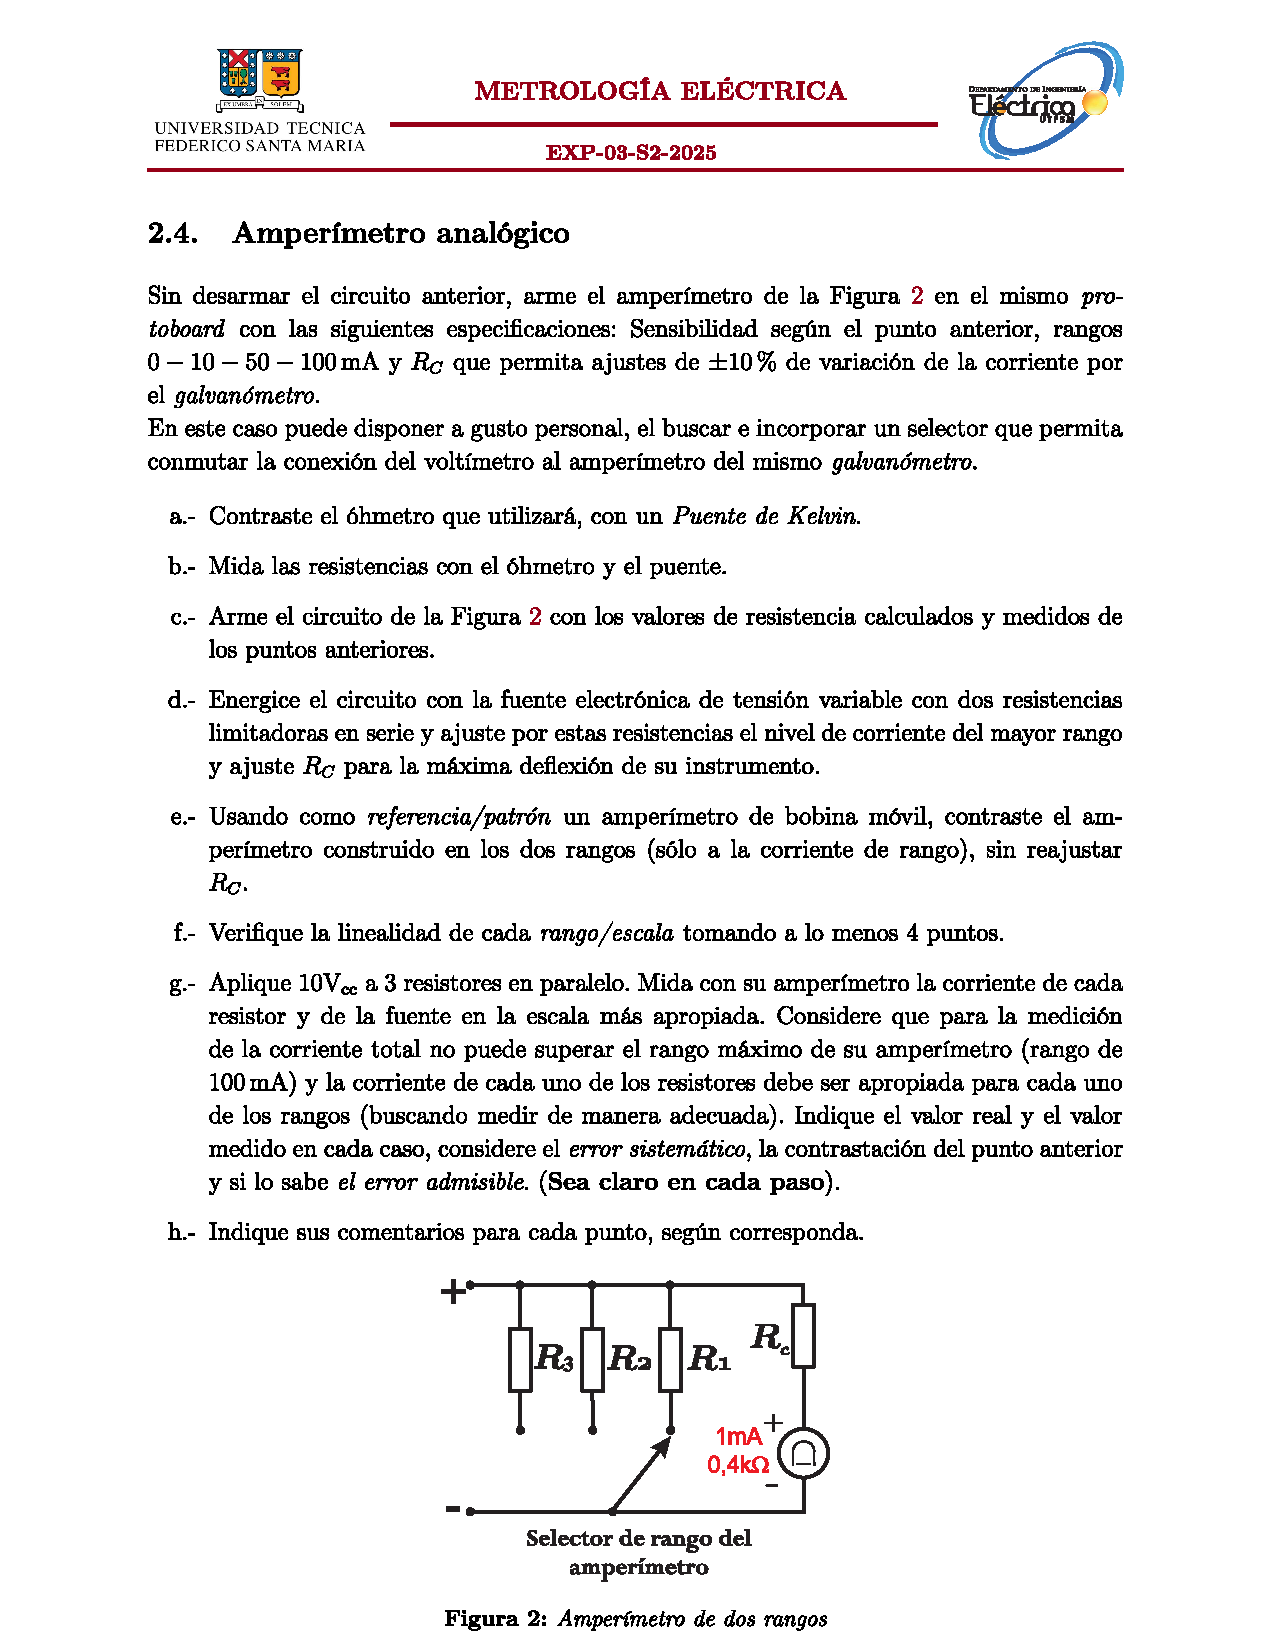
\includegraphics[    angle=0,
    trim=50mm 12mm 50mm 216mm, % izq abajo der arriba
    clip,
    width=\linewidth]{recursos/ammeter.pdf}
  \caption{Esquema circuital del amperímetro de rango variable.}
  \label{fig:ammeter}
\end{figure}

La resistencia de calibración se calcula a partir de la relación entre la corriente que pasa por el galvanómetro $I_g$ y la corriente total $I$ medida por el amperímetro. Usando el cálculo de las resistencias shunt y la ecuación de la corriente a través del galvanómetro, se determina $R_c$ como la resistencia que satisface la relación de corrientes que se desprende del análisis circuital del amperímetro descrito en la figura \ref{fig:ammeter}, tal que:

\[
R_sI - R_sI_g=(R_c+R_g)I_g \Leftrightarrow I = I_g\frac{R_c+R_g+Rs}{R_s}
\]

Donde $I$ corresponde a la corriente máxima a medir en el rango en cuestión, e $I_g$ sea la corriente máxima que es capaz de soportar el galvanómetro.

\subsubsection{Protecciones del Instrumento}
Para proteger al galvanómetro de sobrecorrientes, se incorporan diodos en antiparalelo. Los diodos tienen la característica de que no consumen corriente cuando están en su estado normal, pero cuando la corriente excede un valor umbral (típicamente $0.7 \ [V]/R_g$), los diodos se comportan como cortocircuitos, desviando la corriente y evitando daños en el instrumento.

\subsubsection{Circuito de Contrastación del Amperímetro}
Para verificar el correcto funcionamiento de los rangos diseñados, se implementa un circuito de contrastación. A diferencia de un ajuste tradicional con resistencias variables, en esta experiencia se empleó una resistencia limitadora $R_{lim}$ fija y conocida para cada rango, conectada en serie con el amperímetro bajo prueba y un amperímetro patrón. La variación de corriente, necesaria para tomar múltiples puntos y verificar la linealidad, se logró ajustando la tensión de alimentación de una fuente DC variable desde 10 V hacia abajo. El esquema de este circuito se presenta y diseña en detalle en la sección de trabajo previo.
\subsubsection{Circuito de Validación del Amperímetro}
Con el fin de estudiar el error sistemático del instrumento, se diseñó un circuito de validación compuesto por tres resistencias en paralelo alimentadas por una fuente de 10 V DC. Los valores seleccionados ($R_1 = 1\,\text{k}\Omega$, $R_2 = 330\,\Omega$ y $R_3 = 220\,\Omega$) garantizan que las corrientes de rama sean medibles en los rangos menores (aproximadamente 10 mA, 30 mA y 45 mA respectivamente), mientras que la corriente total del nodo principal no supera el rango máximo de 100 mA del instrumento construido. El esquema y cálculo de este arreglo se detalla en el trabajo previo.
\subsubsection{Puente de Kelvin}
Cuando las resistencias $N$ y $n$ se ajustan de modo que la corriente que fluye por el galvanómetro $G$ tiende a cero, la resistencia desconocida $X$ e expresa mediante la ecuación~\eqref{eq:6.1} de la siguiente forma:

\begin{equation}
X = \frac{N}{M} \times S + \frac{m \times \ell}{m + n + \ell} 
\times \left( \frac{N}{M} - \frac{n}{m} \right)
\label{eq:6.1}
\end{equation}

donde $\ell$ es la resistencia de los conductores de conexión desde el terminal $P_s$ de $S$ hasta el terminal $P_x$ de $X$.

\begin{figure}[H]
    \centering
    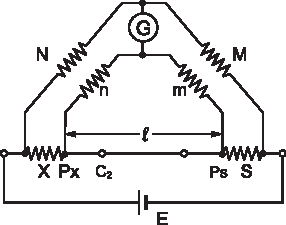
\includegraphics[width=0.5\textwidth]{recursos/kelvin.pdf}
    \caption{Diagrama teórico del circuito del Puente de Kelvin.}
    \label{fig:puente_kelvin}
\end{figure}


El puente de Kelvin está diseñado de modo que las resistencias fijas y las resistencias deslizantes mantienen la siguiente relación:

\[
N = n \quad \text{y} \quad M = m
\]

Por lo tanto:

\[
\frac{N}{M} - \frac{n}{m} = 0
\]

A partir de la ecuación~\eqref{eq:6.1}, se obtiene:

\begin{equation}
X = \frac{N}{M} \times S
\label{eq:6.2}
\end{equation}

Entonces la resistencia baja $X$ puede medirse con gran precisión sin verse afectada por la resistencia de conexión $\ell$.



\newpage
\section{Trabajo Previo}
\subsection{Diseño del Amperímetro de tres rangos}
En esta sección se describen los cálculos realizados para determinar las resistencias de calibración (\( R_c \)) y las resistencias shunt (\( R_{sh} \)) correspondientes a cada rango de medición del amperímetro. Para ello, se utilizó un código en MATLAB que por la facilidad de adaptar los valores de \( R_{sh} \) y \( R_c \) de acuerdo con nuevos requerimientos o con modificaciones sobre la marcha en los valores de la resistencia interna del galvanómetro (\( R_g \)) o de los rangos deseados.

El amperímetro fue diseñado para medir en tres rangos de corriente: 10 mA, 50 mA y 100 mA. Para ello, se fijó una sensibilidad de 700 \(\Omega/V\), lo que implica que la corriente máxima que podría medir el galvanómetro es \( I_m = \frac{1}{s} \), donde \( s \) es la sensibilidad en \(\Omega/V\), la cual debe ser corregida mediante la incorporación de la resistencia de calibración para llevar la corriente máxima al valor aceptado por el galvanómetro de correspondiente a 1 [mA]. 

El cálculo de la resistencia shunt para cada rango de corriente se realizó utilizando la fórmula \ref{eq:Rsh} descrita en el marco teórico, donde \( R_g = 391 \, \Omega \) es la resistencia interna del galvanómetro e \( I_{\text{rango}} \) es la corriente máxima para cada rango.

Del mismo modo, se calcula el valor de la resistencia de calibración necesaria para cada rango a partir de lo expuesto en el marco teórico, junto con determinar el valor que permite un ajuste de +-10\% en la corriente que pasa por el galvanómetro. 

A continuación, se presentan los resultados obtenidos para las resistencias de calibración \( R_c \) y las resistencias shunt \( R_{sh} \) para cada rango de corriente:

\begin{table}[h]
\centering
\caption{Resultados de las resistencias de calibración y shunt para cada rango de corriente.}
\begin{tabular}{|c|c|c|c|c|}
\hline
\textbf{Rango} & \textbf{\( R_{sh} \) [Ohm]}  & \textbf{\( R_c \) [Ohm]} & \textbf{\( R_c \) +10\% [Ohm]} & \textbf{\( R_c \) -10\% [Ohm]} \\ \hline
\textbf{10 mA}  & 65.17 & 195.5 & 260.67 & 130.33 \\ \hline
\textbf{50 mA}  & 11.5 & 172.5  & 230.0  & 115.0  \\ \hline
\textbf{100 mA}  & 5.67 & 170.0 & 226.67 & 113.33 \\ \hline
\end{tabular}
\label{tab:ResitShuntyCal}
\end{table}


\subsection{Simulación}
Para verificar la validez de los cálculos realizados y asegurarse de que el diseño del amperímetro funcione correctamente en los tres rangos, se modeló el sistema en el software de simulación PLECS. En este modelo, se replicó el funcionamiento del galvanómetro y se observaron los resultados en función de las resistencias shunt (\( R_{sh} \)) conectadas en paralelo con el galvanómetro.

El modelo simulado incluye los tres rangos de medición (10 mA, 50 mA y 100 mA), cada uno de los cuales depende de los valores de \( R_{sh} \), ajustados previamente en los cálculos. El diagrama de simulación muestra cómo se conecta el selector de rangos y cómo las resistencias shunt permiten el funcionamiento adecuado del amperímetro a diferentes niveles de corriente.

A continuación se presenta la imagen del circuito simulado en PLECS:

\begin{figure}[h]
    \centering
    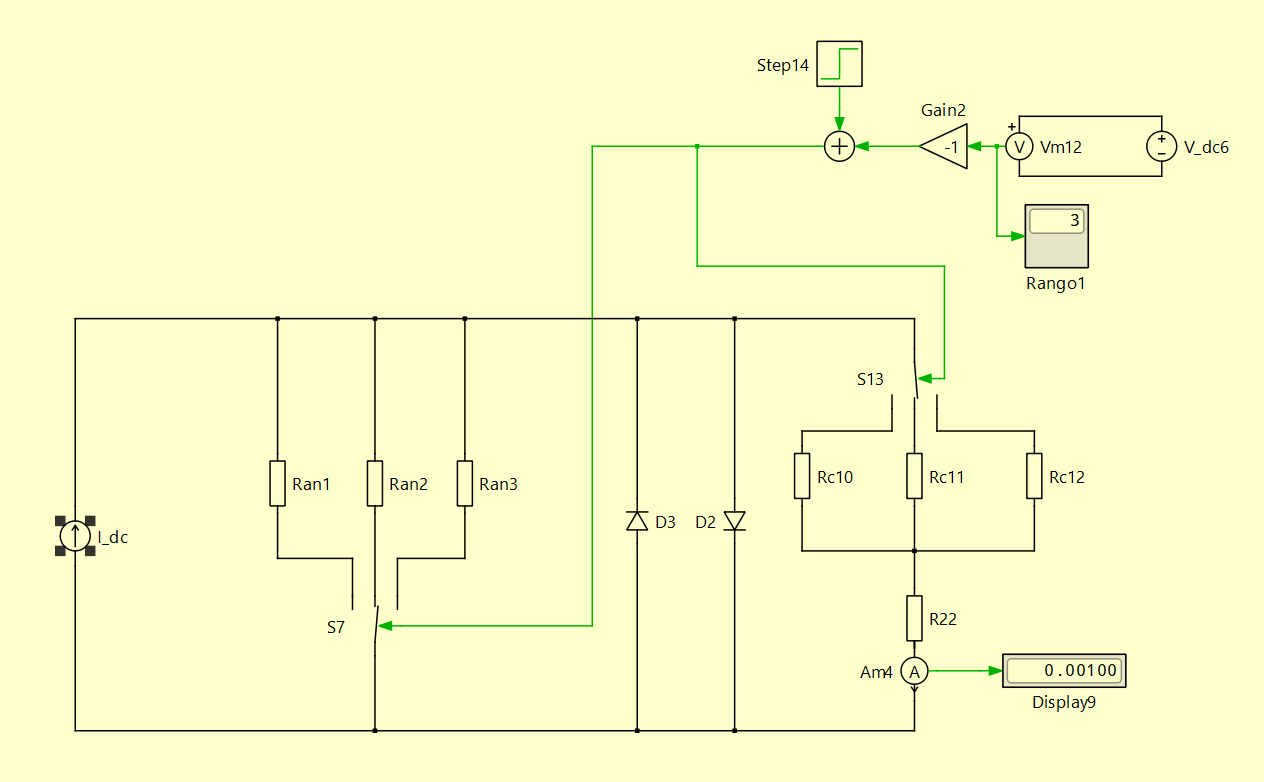
\includegraphics[width=0.7\textwidth]{recursos/imagen_2025-10-22_013807311.png}
    \caption{Modelo del amperímetro en PLECS con tres rangos de corriente dependientes de las resistencias shunt.}
\end{figure}

La simulación mostró que el amperímetro responde correctamente según lo esperado, y los resultados coinciden con los cálculos previos. En cada rango, la corriente medida por el galvanómetro se ajusta adecuadamente, garantizando que las deflexiones de la aguja correspondan a las corrientes máximas especificadas para cada rango de medición.

El ajuste de las resistencias shunt en paralelo con el galvanómetro en la simulación permitió corroborar que el sistema funciona correctamente y que los cálculos realizados para \( R_{sh} \) y \( R_c \) están en línea con el comportamiento teórico del amperímetro.

% --- INICIO DEL CÓDIGO PARA AGREGAR ---


\subsection{Construcción de Resistencias Shunt con Nicrom}
\label{sec:nicrom}

Como parte del trabajo previo, se debe calcular la implementación física de las resistencias shunt ($R_{sh}$). Se sugiere la construcción de estos shunts utilizando alambre de Nicrom, calculando la longitud necesaria del mismo.

Para los cálculos siguientes, se considera un alambre de Nicrom disponible en el pañol, el cual se encuentra rotulado con una resistencia lineal ($\rho_L$) de 5.8 $\Omega$/metro.

La longitud ($L$) requerida para cada resistencia se obtiene dividiendo el valor de resistencia shunt deseado ($R_{sh}$) por la resistividad lineal del alambre ($\rho_L$):
$$ L = \frac{R_{sh}}{\rho_L} $$

Aplicando esta fórmula a los valores de $R_{sh}$ calculados en la Tabla \ref{tab:ResitShuntyCal} (ver sección 4.1), se obtienen las siguientes longitudes de alambre:

\begin{itemize}
    \item \textbf{Rango 1 (10 mA):} Se requiere una $R_{sh1} = 65.16~\Omega$.
        $$ L_1 = \frac{65.16~\Omega}{5.8~\Omega/m} = 11.23~\text{m}$$

    \item \textbf{Rango 2 (50 mA):} Se requiere una $R_{sh2} = 11.5~\Omega$.
        $$ L_2 = \frac{11.5~\Omega}{5.8~\Omega/m} = 1.98~\text{m}$$

    \item \textbf{Rango 3 (100 mA):} Se requiere una $R_{sh3} = 5.66~\Omega$.
        $$ L_3 = \frac{5.66~\Omega}{5.8~\Omega/m} = 0.97~\text{m}$$
\end{itemize}

\newpage
\subsection{Diseño del Circuito de Contrastación}
\label{sec:contrastacion}

Finalmente, la guía solicita diseñar el circuito de contrastación para el instrumento. Para el caso del amperímetro, este circuito debe permitir generar las corrientes de fondo de escala (10 mA, 50 mA y 100 mA) de forma controlada. A diferencia de un método tradicional, en esta experiencia se utilizó una fuente electrónica de tensión de $10~V_{cc}$ variable y solo una resistencia limitadora fija $R_{lim}$ para cada rango, omitiendo el uso de potenciómetros. La variación para obtener los puntos de linealidad se logra ajustando el voltaje de la fuente desde 10 V hacia abajo. El esquema base de este circuito se presenta en la Figura \ref{fig:circuito_prueba_amperimetro}.

\begin{figure}[h!]
  \centering
  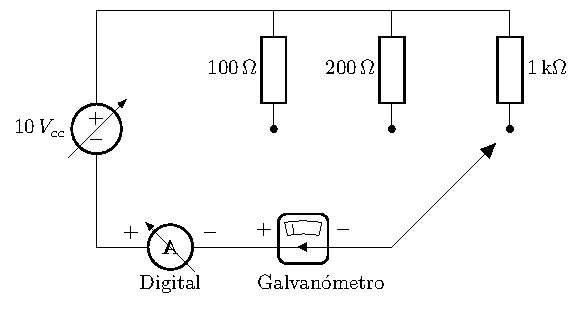
\includegraphics[width=0.7\linewidth]{recursos/circuito_contrastacion.pdf}
    \caption{Esquema del circuito de prueba para la calibración y contrastación del amperímetro empleando resistencia limitadora fija.}
    \label{fig:circuito_prueba_amperimetro}
\end{figure}

Para el cálculo de la resistencia limitadora total ($R_{\text{lim}}$) necesaria para cada rango, se utiliza la Ley de Ohm. Se asume la fuente ajustada a $10~V_{cc}$ y se desprecia la resistencia interna del amperímetro para simplificar la selección de los componentes fijos.

$$ R_{\text{lim}} = \frac{V_{cc}}{I_{\text{rango}}} $$

Los valores de resistencia fija necesarios para alcanzar la corriente de fondo de escala en cada rango a 10 V se resumen en la Tabla \ref{tab:res_prueba}. En la práctica, se implementará esta $R_{\text{lim}}$ mediante una resistencia fija de valor cercano al estándar comercial.

\begin{table}[h!]
    \centering
    \caption{Cálculo de resistencias limitadoras totales para el circuito de prueba con $V_{cc} = 10~V$.}
    \label{tab:res_prueba}
    \begin{tabular}{cccr}
        \toprule
        \textbf{Rango} & \textbf{Rango ($I_{\text{rango}}$)} & \textbf{Fuente ($V_{cc}$)} & \textbf{Resistencia ($R_{\text{lim}}$)} \\
        \midrule
        1 & 10 mA & 10 V & $R_{\text{lim1}} = \frac{10~V}{10~mA} = \mathbf{1~k\Omega}$ \\
        2 & 50 mA & 10 V & $R_{\text{lim2}} = \frac{10~V}{50~mA} = \mathbf{200~\Omega}$ \\
        3 & 100 mA & 10 V & $R_{\text{lim3}} = \frac{10~V}{100~mA} = \mathbf{100~\Omega}$ \\
        \bottomrule
    \end{tabular}
\end{table}

\newpage
\subsection{Diseño del Circuito de Carga en Paralelo}
\label{sec:paralelo}

Adicionalmente, se solicita en la guía de la experiencia (punto 2.4.g) la aplicación de $10~V_{cc}$ a tres resistores en paralelo, para medir tanto la corriente de cada resistor como la corriente de la fuente, utilizando los rangos apropiados del amperímetro construido.

Para esto, se diseñó un circuito de carga como el mostrado en la Figura \ref{fig:circuito_paralelo}, alimentado por una fuente $V_{cc}$ de 10 V. El objetivo es que la corriente total ($I_{\text{fuente}}$) sea de 100 mA, correspondiente al rango máximo del instrumento, y que las corrientes individuales ($I_1$, $I_2$, $I_3$) se distribuyan de forma que puedan medirse con los distintos rangos (100 mA, 50 mA y 10 mA).

\begin{figure}[h!]
  \centering
  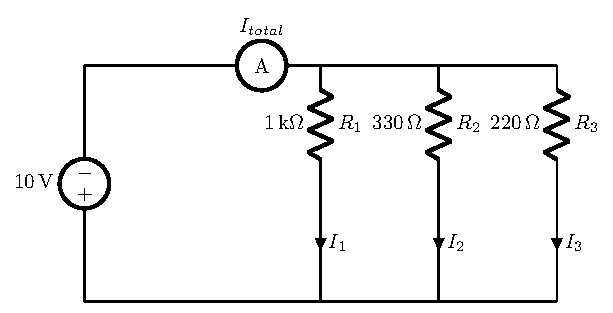
\includegraphics[width=0.7\linewidth]{recursos/circuito_validacion.pdf}
    \caption{Esquema del circuito de prueba con carga en paralelo.}
    \label{fig:circuito_paralelo}
\end{figure}

Se buscaron valores de resistencia comerciales que, asumiendo una tensión ideal de 10 V en sus terminales, generaran las corrientes deseadas dentro de los rangos del instrumento. Los valores seleccionados se resumen en la Tabla \ref{tab:res_paralelo}.

\begin{table}[h!]
    \centering
    \caption{Resistencias de carga en paralelo y corrientes teóricas.}
    \label{tab:res_paralelo}
    \begin{tabular}{cccl}
        \toprule
        \textbf{Componente} & \textbf{Corriente teórica $I_n$} & \textbf{Resistencia seleccionada $R_n$} & \textbf{Rango a Utilizar} \\
        \midrule
        $R_1$ & 10 mA & 1 k$\Omega$ & 10 mA \\
        $R_2$ & 30.3 mA & 330 $\Omega$ & 50 mA \\
        $R_3$ & 45.4 mA & 220 $\Omega$ & 50 mA \\
        \midrule
        Total & $\sim$ 85.7 mA & - & 100 mA \\
        \bottomrule
    \end{tabular}
\end{table}

\newpage
Según el diseño, la corriente total que debe entregar la fuente es la suma de las corrientes individuales:
$$ I_{\text{fuente}} = I_1 + I_2 + I_3 = 10~\text{mA} + 30.3~\text{mA} + 45.4~\text{mA} \approx 85.7~\text{mA} $$
Este valor es inferior a los 100 mA del rango máximo del amperímetro, garantizando una validación segura del instrumento sin riesgo de sobrecorriente.

\newpage
\section{Desarrollo de la Experiencia}
\label{sec:desarrollo}

Para la implementación práctica del amperímetro, se utilizó la metodología descrita en la guía de la experiencia, complementada con los cálculos del trabajo previo. El procedimiento se dividió en dos etapas principales: la calibración del instrumento y la prueba en un circuito de carga.

\subsection{Armado y Calibración del Amperímetro}

El montaje experimental se realizó utilizando dos protoboards. En uno se ensambló el amperímetro analógico, conectando el galvanómetro, la resistencia de calibración $R_c$ y las tres resistencias shunt ($R_{sh1}$, $R_{sh2}$, $R_{sh3}$) calculadas, junto al selector de rango. En el segundo protoboard se montó el circuito de prueba (o contrastación), compuesto por la fuente de $10~V_{cc}$ variable y las resistencias limitadoras fijas calculadas en la sección \ref{sec:contrastacion}.

Para la calibración, se procedió de la siguiente manera:
\begin{enumerate}
    \item Se construyó $R_{sh2} = 11.5~\Omega$ y $R_{sh3} = 5.66~\Omega$ enrrollando alambre de nicrom en un lápiz. Se usó una resistencia en $R_{sh1} = 65.16~\Omega$ para evitar enrrollar 12 metros de alambre.
    \item Se contrastaron las mediciones de las resistencias $R_{sh2}$ y $R_{sh3}$ obtenidas con multímetro digital mediante el uso de un Puente de Kelvin.
    \item Se colocó un multímetro digital en modo amperímetro, actuando como instrumento patrón, en serie con el amperímetro analógico a construir.
    \item Se seleccionó el rango máximo del instrumento (100 mA) y se conectó la resistencia limitadora correspondiente al rango.
    \item Se energizó el circuito de prueba y se ajustó el nivel de tensión de la fuente hasta que el instrumento patrón indicó una corriente exacta de 100 mA.
    \item Sobre esta condición, se ajustó la resistencia de calibración $R_c$ del amperímetro analógico hasta que la aguja del galvanómetro alcanzó la máxima deflexión (fondo de escala).
    \item Luego, se modificó el circuito de prueba para suministrar 50 mA (medidos por el patrón) y se seleccionó el rango de 50 mA en el amperímetro analógico. Se registró la medición sin reajustar $R_c$, con el fin de medir el error inducido por la calibración única.
    \item Se repitió el paso anterior para el rango de 10 mA, ajustando la fuente de prueba a 10 mA.
\end{enumerate}

\subsection{Medición en Circuito de Carga en Paralelo}

Una vez calibrado el instrumento, se procedió a armar el circuito de carga en paralelo diseñado en la sección \ref{sec:paralelo}. Para conseguir los valores de resistencia $R_1$, $R_2$ y $R_3$ (1 k$\Omega$, 330 $\Omega$ y 220 $\Omega$), se utilizaron resistores de valores comerciales.

Se realizaron las siguientes mediciones, siempre manteniendo el multímetro patrón en serie con el amperímetro analógico para contrastar los resultados:
\begin{enumerate}
    \item Se midió la corriente total $I_{\text{fuente}}$, insertando los amperímetros entre la fuente $V_{cc}$ y el nodo común de las resistencias en paralelo.
    \item Se midió la corriente individual $I_1$, $I_2$ e $I_3$ que circula por cada resistencia, insertando los instrumentos en serie con cada rama correspondiente.
\end{enumerate}

Finalmente, los valores medidos por el amperímetro analógico fueron comparados con la medición del instrumento patrón y con el valor teórico esperado ($V_{cc}/R$).



\section{Resultados}
% --- INICIO DEL CÓDIGO PARA AGREGAR ---
% (Asegúrate de tener \usepackage{booktabs} en tu preámbulo)


En esta sección se presentan los resultados obtenidos del montaje práctico del amperímetro. Mencionar que durante la etapa de calibración inicial, el potenciómetro destinado al ajuste de $R_c$ (resistencia de calibración) sufrió una falla, quemándose e impidiendo su ajuste posterior. 

Debido a este inconveniente, con autorización del profesor, se hizo variar la fuente de voltaje para controlar la corriente que pasaba por el circuito considerando solo la resistencia de 100 $\Omega$ contemplada en el diseño del circuito de calibración. Por lo mismo, para las pruebas de linealidad, en lugar de ajustar la resistencia de prueba con el potenciómetro, se optó por variar directamente la tensión de la fuente ($V_{cc}$) para generar las distintas corrientes de prueba, las cuales fueron monitoreadas en todo momento por el multímetro digital actuando como patrón.

\subsection{Calibración y Error de Rango}

La calibración se realizó exitosamente para el rango de 100 mA. Se ajustó la fuente hasta que el multímetro patrón midió 100 mA, y en ese punto se ajustó $R_c$ hasta que la aguja del galvanómetro indicó plena escala.

Luego, con ese valor de $R_c$ fijo, se procedió a medir el error en los otros rangos. Para ello, se ajustó la fuente de tensión hasta que el amperímetro construido marcó el fondo de escala (50 mA y 10 mA, respectivamente) y se registró la corriente real que estaba midiendo el patrón. Los resultados se resumen en la Tabla \ref{tab:calibracion}.

\begin{table}[h!]
    \centering
    \caption{Contrastación de fondo de escala con $R_c$ fija (calibrada para 100 mA). Los datos provienen de la hoja de resultados (Imagen 2).}
    \label{tab:calibracion}
    \begin{tabular}{cccc}
        \toprule
        \textbf{$V_{cc}$} & 
        \textbf{Rango} & \textbf{Lectura Amperímetro} & \textbf{Patrón} \\
        \midrule
        11 & 100 mA & 100 mA & 100 mA \\
        7 & 50 mA & 50 mA & 58.6 mA \\
        1,9 & 10 mA & 10 mA & 11.64 mA \\
        \bottomrule
    \end{tabular}
\end{table}

Se observa un error considerable en los rangos inferiores, lo cual era esperado, ya que el valor de $R_c$ óptimo es distinto para cada rango (como se calculó en el Trabajo Previo), pero en la práctica se utilizó un valor único fijado para el rango mayor.

Los cálculos del error son los siguientes:
\begin{itemize}
\item \textbf{Rango 100 mA:} El error es $0.0\%$, ya que este fue el punto de calibración.
\item \textbf{Rango 50 mA:} $\text{Error \%} = \frac{|50 - 58.6|}{58.6} \times 100\% = 14.67\%$.
\item \textbf{Rango 10 mA:} $\text{Error \%} = \frac{|10 - 11.64|}{11.64} \times 100\% = 14.09\%$.
\end{itemize}

Estos resultados demuestran que el instrumento, al ser calibrado para el rango máximo, subestima considerablemente la corriente en los rangos inferiores. Es decir, para que la aguja marque "50 mA", se requiere una corriente real de 58.6 mA por ejemplo.

\subsection{Verificación de Linealidad}

Posteriormente, se verificó la linealidad de cada rango variando la tensión de la fuente para obtener distintos puntos de medición. Las Tablas \ref{tab:lin100}, \ref{tab:lin50} y \ref{tab:lin10} (basadas en la Imagen 1) comparan la lectura del patrón (DMM) con la del amperímetro construido.

\begin{table}[h!]
    \centering
    \caption{Linealidad del Rango 100 mA.}
    \label{tab:lin100}
    \begin{tabular}{ccc}
        \toprule
        \textbf{Tensión Fuente (V)} & \textbf{Corriente Patrón (mA)} & \textbf{Lectura Amperímetro (mA)} \\
        \midrule
        10.0 & 92.8 & 94.5 \\
        8.0 & 73.5 & 78 \\
        5.4 & 48.8 & 56 \\
        3.3 & 30.79 & 36 \\
        \bottomrule
    \end{tabular}
\end{table}

\begin{table}[h!]
    \centering
    \caption{Linealidad del Rango 50 mA.}
    \label{tab:lin50}
    \begin{tabular}{ccc}
        \toprule
        \textbf{Tensión Fuente (V)} & \textbf{Corriente Patrón (mA)} & \textbf{Lectura Amperímetro (mA)} \\
        \midrule
        5.6 & 48.8 & 50 \\
        3.8 & 33.39 & 36 \\
        2.5 & 22.36 & 26 \\
        1.1 & 9.95 & 12 \\
        \bottomrule
    \end{tabular}
\end{table}

\begin{table}[h!]
    \centering
    \caption{Linealidad del Rango 10 mA.}
    \label{tab:lin10}
    \begin{tabular}{ccc}
        \toprule
        \textbf{Tensión Fuente (V)} & \textbf{Corriente Patrón (mA)} & \textbf{Lectura Amperímetro (mA)} \\
        \midrule
        1.5 & 9.55 & 10 \\
        1.2 & 7.58 & 8 \\
        0.6 & 4.02 & 4.6 \\
        0.2 & 1.71 & 2 \\
        \bottomrule
    \end{tabular}
\end{table}

\subsubsection{Análisis Gráfico de Linealidad}

Para analizar visualmente la linealidad del instrumento, se graficó la corriente medida por el amperímetro construido ($I_a$) en función de la corriente real medida por el patrón ($I_p$). El resultado se presenta en la Figura \ref{fig:linealidad_amp}.

\begin{figure}[h!]
    \centering
    \includesvg[width=0.80\textwidth]{recursos/LinAmp.svg}
    \caption{Gráfico de linealidad $I_a$ vs. $I_p$ para los tres rangos,
    con sus respectivos ajustes lineales ($I_a = m \cdot I_p + b$) y
    coeficientes de determinación ($R^2$).}
    \label{fig:linealidad_amp}
\end{figure}

Del gráfico se puede extraer que, tal como se esperaba, existe un comportamiento claramente lineal en los tres rangos. Esto se confirma cuantitativamente con los coeficientes de determinación ($R^2$), que en todos los casos son superiores a 0.996, indicando un ajuste lineal casi perfecto. Este comportamiento se fundamenta en el marco teórico, ya que la corriente que circula por el galvanómetro ($I_g$) es linealmente proporcional a la corriente total del circuito ($I_p$) a través de un factor constante para cada rango, dado por las resistencias $R_g$, $R_{sh}$ y $R_c$. La lectura final del amperímetro ($I_a$) es, a su vez, la corriente $I_g$ multiplicada por un factor de escala constante (ej. 100 en el rango de 100 mA, 50 en el de 50 mA, etc.). Por lo tanto, la relación entre la lectura $I_a$ y la corriente patrón $I_p$ debe ser lineal, siguiendo la ecuación $I_a = m \cdot I_p + b$.

Sin embargo, al analizar los coeficientes específicos del ajuste, se observa una situación bastante anómala. El rango de 10 mA presenta un comportamiento casi ideal, con una pendiente $m=1.01$ (muy cercana a 1) y un intercepto $b=0.38$ mA (muy cercano a 0). En contraste directo, el rango de 100 mA, que supuestamente fue el rango utilizado para la calibración inicial (Sección 6.1), muestra la mayor desviación: una pendiente $m=0.94$ y un gran intercepto $b=8.62$ mA. El rango de 50 mA también presenta un offset considerable ($b=3.23$ mA).

Esta fuerte discrepancia sugiere una fuente de error externa que va más allá del uso de un solo $R_c$. Los datos del gráfico de linealidad contradicen la calibración reportada. Es altamente probable que, en algún momento entre la calibración inicial (donde se ajustó $R_c$ para 100 mA) y la ejecución de estas pruebas de linealidad, el instrumento haya sido recalibrado, intencional o accidentalmente, para que la plena escala coincidiera con el rango de 10 mA. Esto explicaría por qué el ajuste del rango de 10 mA es casi perfecto, mientras que los rangos superiores, especialmente el de 100 mA, heredan un error sistemático tan significativo.

\subsection{Prueba en Circuito de Carga Paralelo}

Finalmente, se implementó el circuito de carga en paralelo (diseñado en la sección \ref{sec:paralelo}) para simular una situación de medición real. Se midió la corriente en cada rama ($R_1, R_2, R_3$) y la corriente total de la fuente.

Para estas mediciones, se utilizaron los valores de resistencia calculados en el trabajo previo ($R_1=1\text{ k}\Omega$, $R_2=330~\Omega$, $R_3=220~\Omega$). Los valores teóricos de corriente (asumiendo $V_{cc}=10~V$) son: $I_1 = 10.0$ mA, $I_2 = 30.3$ mA, $I_3 = 45.4$ mA, y $I_{\text{Fuente}} \approx 85.7$ mA.

La Tabla \ref{tab:paralelo} (basada en los datos simulados a partir de las mediciones del patrón) resume los resultados, donde se contrasta la lectura del amperímetro construido y la del patrón al medir en cada rama.

\begin{table}[h!]
    \centering
    \caption{Mediciones en Circuito de Carga Paralelo.}
    \label{tab:paralelo}
    \begin{tabular}{cccc}
        \toprule
        \makecell{\textbf{Elemento}\\\textbf{Medido}\\\textbf{(Teórico)}} & 
        \makecell{\textbf{Rango}\\\textbf{Usado}} & 
        \makecell{\textbf{Corriente}\\\textbf{Patrón}\\\textbf{(mA)}} & 
        \makecell{\textbf{Lectura}\\\textbf{Amperímetro}\\\textbf{(mA)}} \\
        \midrule
        $R_1$ (10.0 mA) & 10 mA & 8.1 & 8.6 \\
        $R_1$ (10.0 mA) & 50 mA & 8.5 & 11.5 \\
        \midrule
        $R_2$ (30.3 mA) & 50 mA & 19.6 & 22.0 \\
        $R_2$ (30.3 mA) & 100 mA & 19.8 & 27.0 \\
        \midrule
        $R_3$ (45.4 mA) & 50 mA & 24.9 & 27.5 \\
        $R_3$ (45.4 mA) & 100 mA & 25.3 & 32.0 \\
        \midrule
        $I_{\text{Fuente}}$ (85.7 mA) & 100 mA & 34.3 & 41.0 \\
        \bottomrule
    \end{tabular}
\end{table}


Es de gran interés observar el efecto de carga del instrumento. Por ejemplo, al medir la corriente en $R_1$ (teórica 10.0 mA), el patrón mide 8.1 mA cuando se usa el rango de 10 mA del amperímetro, pero mide 8.5 mA cuando se usa el rango de 50 mA. Esto se debe a que la resistencia interna del amperímetro ($R_A$) cambia con el rango seleccionado, perturbando el circuito de forma distinta en cada caso.

\subsubsection{Análisis de Error y Efecto de Carga}

A partir de los datos de la Tabla \ref{tab:paralelo}, se pueden realizar dos análisis de error distintos. Primero, se analiza el error de nuestro amperímetro construido, comparando su lectura ($I_a$) con el valor real dado por el patrón ($I_p$). El error porcentual se calcula como $\text{Error \%} = \frac{|I_a - I_p|}{I_p} \times 100\%$. Los resultados se resumen en la Tabla \ref{tab:paralelo_error_medicion}.

\begin{table}[h!]
    \centering
    \caption{Error de Medición del amperímetro (Lectura vs. Patrón).}
    \label{tab:paralelo_error_medicion}
    \begin{tabular}{ccccc}
        \toprule
        \textbf{Elemento} & \textbf{Rango} & \textbf{Patrón ($I_p$)} & \textbf{Lectura ($I_a$)} & \textbf{Error \%} \\
        \midrule
        $R_1$ & 10 mA & 8.1 mA & 8.6 mA & 6.17 \% \\
        $R_1$ & 50 mA & 8.5 mA & 11.5 mA & 35.29 \% \\
        \midrule
        $R_2$ & 50 mA & 19.6 mA & 22.0 mA & 12.24 \% \\
        $R_2$ & 100 mA & 19.8 mA & 27.0 mA & 36.36 \% \\
        \midrule        
        $R_3$ & 50 mA & 24.9 mA & 27.5 mA & 10.44 \% \\
        $R_3$ & 100 mA & 25.3 mA & 32.0 mA & 26.48 \% \\
        \midrule
        $I_{\text{Fuente}}$ & 100 mA & 34.3 mA & 41.0 mA & 19.53 \% \\
        \bottomrule
    \end{tabular}
\end{table}

Las mediciones del amperímetro construido presentan errores considerables, particularmente acentuados en los rangos superiores (50 mA y 100 mA). Esto es coherente con los resultados de la calibración y el análisis de linealidad (el fuerte "offset" o intercepto $b$), confirmando que el instrumento arrastra un error sistemático grande para esas escalas, mientras que en el rango de 10 mA el error se mantiene relativamente bajo (alrededor del 6\%).

\newpage
En segundo lugar, se analiza el efecto de carga o la perturbación que nuestro amperímetro introduce en el circuito. Para esto, comparamos la corriente teórica que debería fluir por la rama (ej. $I_{\text{teo}} = 10V / R_1$) con la corriente real que fluyó una vez que el amperímetro fue insertado (medida por el patrón, $I_p$). El error porcentual se calcula como $\text{Error \%} = \frac{|I_p - I_{\text{teo}}|}{I_{\text{teo}}} \times 100\%$.

\begin{table}[h!]
    \centering
    \caption{Efecto de Carga (Perturbación del Sistema).}
    \label{tab:paralelo_error_carga}
    \begin{tabular}{ccccc}
        \toprule
        \textbf{Elemento} & \textbf{Teórico ($I_{\text{teo}}$)} & \textbf{Rango Usado} & \textbf{Patrón ($I_p$)} & \textbf{Perturbación \%} \\
        \midrule
        $R_1$ & 10.0 mA & 10 mA & 8.1 mA & 19.00 \% \\
        $R_1$ & 10.0 mA & 50 mA & 8.5 mA & 15.00 \% \\
        \midrule
        $R_2$ & 30.3 mA & 50 mA & 19.6 mA & 35.31 \% \\
        $R_2$ & 30.3 mA & 100 mA & 19.8 mA & 34.65 \% \\
        \midrule
        $R_3$ & 45.4 mA & 50 mA & 24.9 mA & 45.15 \% \\
        $R_3$ & 45.4 mA & 100 mA & 25.3 mA & 44.27 \% \\
        \midrule
        $I_{\text{Fuente}}$ & 85.7 mA & 100 mA & 34.3 mA & 59.98 \% \\
        \bottomrule
    \end{tabular}
\end{table}

A partir de la tabla \ref{tab:paralelo_error_carga} se observa un fenómeno sumamente revelador: la introducción del amperímetro perturba el circuito de manera masiva. Las perturbaciones varían desde un 15\% hasta casi un 60\% en el caso de la medición de la corriente total de la fuente. 

Por diseño, un amperímetro inserta una resistencia interna ($R_A$) en serie con el tramo donde mide. En nuestro diseño, debido a la resistencia limitadora de 100 $\Omega$ que domina el ajuste, la $R_A$ resultante es muy alta (del orden de 170-220 $\Omega$ dependiendo del rango). Al intentar medir ramas de baja resistencia, como $R_2$ (330 $\Omega$) o $R_3$ (220 $\Omega$), o al poner el instrumento en serie con la fuente ($R_{\text{eq}} \approx 116\text{ }\Omega$), el instrumento casi duplica la resistencia total de la rama, causando caídas abruptas en la corriente real ($I_p$).

Esto ilustra perfectamente el principio de efecto de carga: el acto de medir altera de manera drástica el circuito si el instrumento no cuenta con una impedancia ideal (en este caso, una $R_A$ que debiese tender a cero). Además, se aprecia que los distintos rangos (con distintas $R_A$) introducen niveles ligeramente diferentes de perturbación.









\subsection{Error escala lineal}



 Error corregido por calibración (error de exactitud): 
Si se utiliza la ecuación inversa de la recta de ajuste como función de calibración, se puede estimar la corriente patrón real a partir de una lectura del instrumento:

\begin{equation}
I_{a,\text{corr}} = \frac{I_a - b}{m}
\end{equation}

y definir el error de exactitud corregido como:

\begin{equation}
\varepsilon_{\text{cal}} (\%) = 
\frac{\left| I_{a,\text{corr}} - I_p \right|}{I_p} \times 100
\end{equation}

Este error refleja la precisión real del instrumento una vez que sus desviaciones sistemáticas son neutralizadas matemáticamente mediante el modelo lineal obtenido en las pruebas previas.

\begin{table}[h!]
    \centering
    \caption{Coeficientes del ajuste lineal para cada rango del amperímetro.}
    \label{tab:coeficientes_lineales}
    \begin{tabular}{ccc}
        \toprule
        \makecell{\textbf{Rango}} &
        \makecell{\textbf{Pendiente}\\$(m)$} &
        \makecell{\textbf{Intercepto}\\$(b)$ (mA)} \\
        \midrule
        100 mA & 0.94 & 8.62 \\
        50 mA  & 0.97 & 3.23 \\
        10 mA  & 1.01 & 0.38 \\
        \bottomrule
    \end{tabular}
\end{table}

\begin{table}[h!]
    \centering
    \caption{Mediciones en circuito de carga paralelo con corrección matemática lineal.}
    \label{tab:paralelo_corr3}
    \begin{tabular}{cccccc}
        \toprule
        \makecell{\textbf{Elemento}\\\textbf{Medido}\\\textbf{(Teórico)}} &
        \makecell{\textbf{Rango}\\\textbf{Usado}} &
        \makecell{\textbf{Corriente}\\\textbf{Patrón}\\\textbf{(mA)}} &
        \makecell{\textbf{Lectura}\\\textbf{Amperímetro}\\\textbf{(mA)}} &
        \makecell{\textbf{Valor}\\\textbf{Corregido}\\\textbf{$I_{a,\text{corr}}$ (mA)}} &
        \makecell{\textbf{Error}\\\textbf{corregido}\\\textbf{(\%)}} \\
        \midrule
        $R_1$ (10.0 mA) & 10 mA  & 8.1  & 8.6  & 8.14  & 0.49 \\
        $R_1$ (10.0 mA) & 50 mA  & 8.5  & 11.5 & 8.53  & 0.35 \\
        \midrule
        $R_2$ (30.3 mA) & 50 mA  & 19.6 & 22.0 & 19.35 & 1.28 \\
        $R_2$ (30.3 mA) & 100 mA & 19.8 & 27.0 & 19.55 & 1.26 \\
        \midrule
        $R_3$ (45.4 mA) & 50 mA  & 24.9 & 27.5 & 25.02 & 0.48 \\
        $R_3$ (45.4 mA) & 100 mA & 25.3 & 32.0 & 24.87 & 1.70 \\
        \midrule
        $I_{\text{Fuente}}$ (85.7 mA) & 100 mA & 34.3 & 41.0 & 34.45 & 0.44 \\
        \bottomrule
    \end{tabular}
\end{table}

Los resultados de la Tabla \ref{tab:paralelo_corr3} validan de manera contundente la estrategia de corrección. Mientras que los errores crudos en la Tabla 7 llegaban hasta el 36\%, la corrección lineal es capaz de reducir el error de exactitud por debajo del 2\% en todos los casos. Esto demuestra que el instrumento, pese a sus enormes offsets sistemáticos y efecto de carga (problemas de exactitud e interacción con el sistema), goza de una precisión y repetibilidad (linealidad) excelentes, permitiendo reconstruir el valor real con alta confiabilidad a través de una función de transferencia inversa.





% --- FIN DEL CÓDIGO PARA AGREGAR ---

\newpage
\section{Conclusiones}
\label{sec:conclusiones}

El desarrollo de esta experiencia permitió cumplir satisfactoriamente con los objetivos planteados, centrados en la construcción, análisis y validación de un amperímetro analógico multirrango, a pesar de las adaptaciones metodológicas forzadas por fallas en el equipamiento (potenciómetros). 

El cambio de metodología, utilizando una resistencia limitadora fija y variando la tensión de la fuente, demostró que es posible contrastar y verificar la linealidad del instrumento. Sin embargo, al depender de una única resistencia de calibración ($R_c$) optimizada empíricamente para el rango de 100 mA, se evidenció que los rangos inferiores sufren un error sistemático inherente debido a que no operan en su punto óptimo de sintonía.

En cuanto a la linealidad, se comprobó experimentalmente que el diseño basado en divisores resistivos (shunt) mantiene un comportamiento lineal casi perfecto ($R^2 > 0.996$ en todos los rangos). No obstante, el fuerte "offset" o intercepto observado en las curvas de calibración de los rangos superiores confirma la presencia de un marcado error de exactitud. Esto subraya que la linealidad (precisión y proporcionalidad) no garantiza la exactitud si la calibración del punto cero u offset es inadecuada.

El análisis del circuito de carga en paralelo fue fundamental para ilustrar el \textit{efecto de carga} y la naturaleza intrusiva de la medición de corriente. Al utilizar la fuente de 10 V con las nuevas resistencias ($1\text{ k}\Omega, 330\text{ }\Omega, 220\text{ }\Omega$), se observó una perturbación extrema del circuito. Dado que el amperímetro presentaba una alta resistencia interna (producto de las adaptaciones del circuito de calibración), la mera inserción del instrumento duplicó la resistencia total en varias ramas, provocando caídas de la corriente real de hasta un 60\% respecto al valor teórico esperado (ver Tabla \ref{tab:paralelo_error_carga}). Esto resalta drásticamente la importancia crítica de diseñar amperímetros con una impedancia interna que tienda a cero, para evitar desvirtuar la magnitud que se intenta medir.

Finalmente, el análisis de error y su posterior mitigación matemática validaron la robustez del modelo lineal. Aunque el amperímetro presentaba errores brutos de lectura superiores al 36\% debido a su offset y efecto de carga, el uso de la ecuación inversa de la recta de calibración ($I_{a,\text{corr}} = \frac{I_a - b}{m}$) permitió reconstruir el valor verdadero de la corriente con un error corregido inferior al 2\% en todos los casos. Esto demuestra que, siempre y cuando un instrumento sea rigurosamente lineal y repetible, sus deficiencias de exactitud sistemática pueden ser suprimidas exitosamente mediante una caracterización y compensación matemática adecuada.

%\newpage
%\section{Anexos}
%\subsection{Código MATLAB para dimensionamiento de $R_s$ y $R_c$}

%\addcontentsline{toc}{section}{Apéndice A. Código MATLAB}

\begin{lstlisting}[caption={Cálculo de resistencias Shunt $R_s$ y de calibración $R_c$ para un amperímetro de bobina móvil de tres rangos},label={lst:matlab_voltimetro}]
syms Rc Ig
s = 700; Rg = 391;
Rango1 = 10e-3; Rango2 = 50e-3; Rango3 = 100e-3;
Isen = 1/s;

Rsh1 = Rg * Isen/(Rango1-Isen);
Rsh2 = Rg * Isen/(Rango2-Isen);
Rsh3 = Rg * Isen/(Rango3-Isen);

I1 = @(Ig) Ig * (1+(Rc+Rg)/Rsh1);
I2 = @(Ig) Ig * (1+(Rc+Rg)/Rsh2);
I3 = @(Ig) Ig * (1+(Rc+Rg)/Rsh3);

expr = I1(1e-3); %Cuando mide la corriente maxima, está midiendo la corrinte de rango 1
eq = expr == Rango1; a = vpasolve(eq, Rc);
disp("El valor para rango 1 de Rc es: " + string(a));
eq = expr == Rango1*1.1; a = vpasolve(eq, Rc);
disp("Para +10%: " + string(a));
eq = expr == Rango1*0.9;
a = vpasolve(eq, Rc);
disp("Para -10%: " + string(a));
disp("Y el de Rsh: " + string(Rsh1));

expr = I2(1e-3); %Cuando mide la corriente maxima, está midiendo la corrinte de rango 2
eq = expr == Rango2; a = vpasolve(eq, Rc);
disp("El valor para rango 2 de Rc es: " + string(a));
eq = expr == Rango2*1.1; a = vpasolve(eq, Rc);
disp("Para +10%: " + string(a));
eq = expr == Rango2*0.9; a = vpasolve(eq, Rc);
disp("Para -10%: " + string(a));
disp("Y el de Rsh: " + string(Rsh2));

expr = I3(1e-3); %Cuando mide la corriente maxima, está midiendo la corrinte de rango 3
eq = expr == Rango3; a = vpasolve(eq, Rc);
disp("El valor para rango 3 de Rc es: " + string(a));
eq = expr == Rango3*1.1; a = vpasolve(eq, Rc);
disp("Para +10%: " + string(a));
eq = expr == Rango3*0.9; a = vpasolve(eq, Rc);
disp("Para -10%: " + string(a));
disp("Y el de Rsh: " + string(Rsh3));
\end{lstlisting}



\subsection{Imágenes cuaderno de preinforme}

\begin{figure}[H]
    \centering
    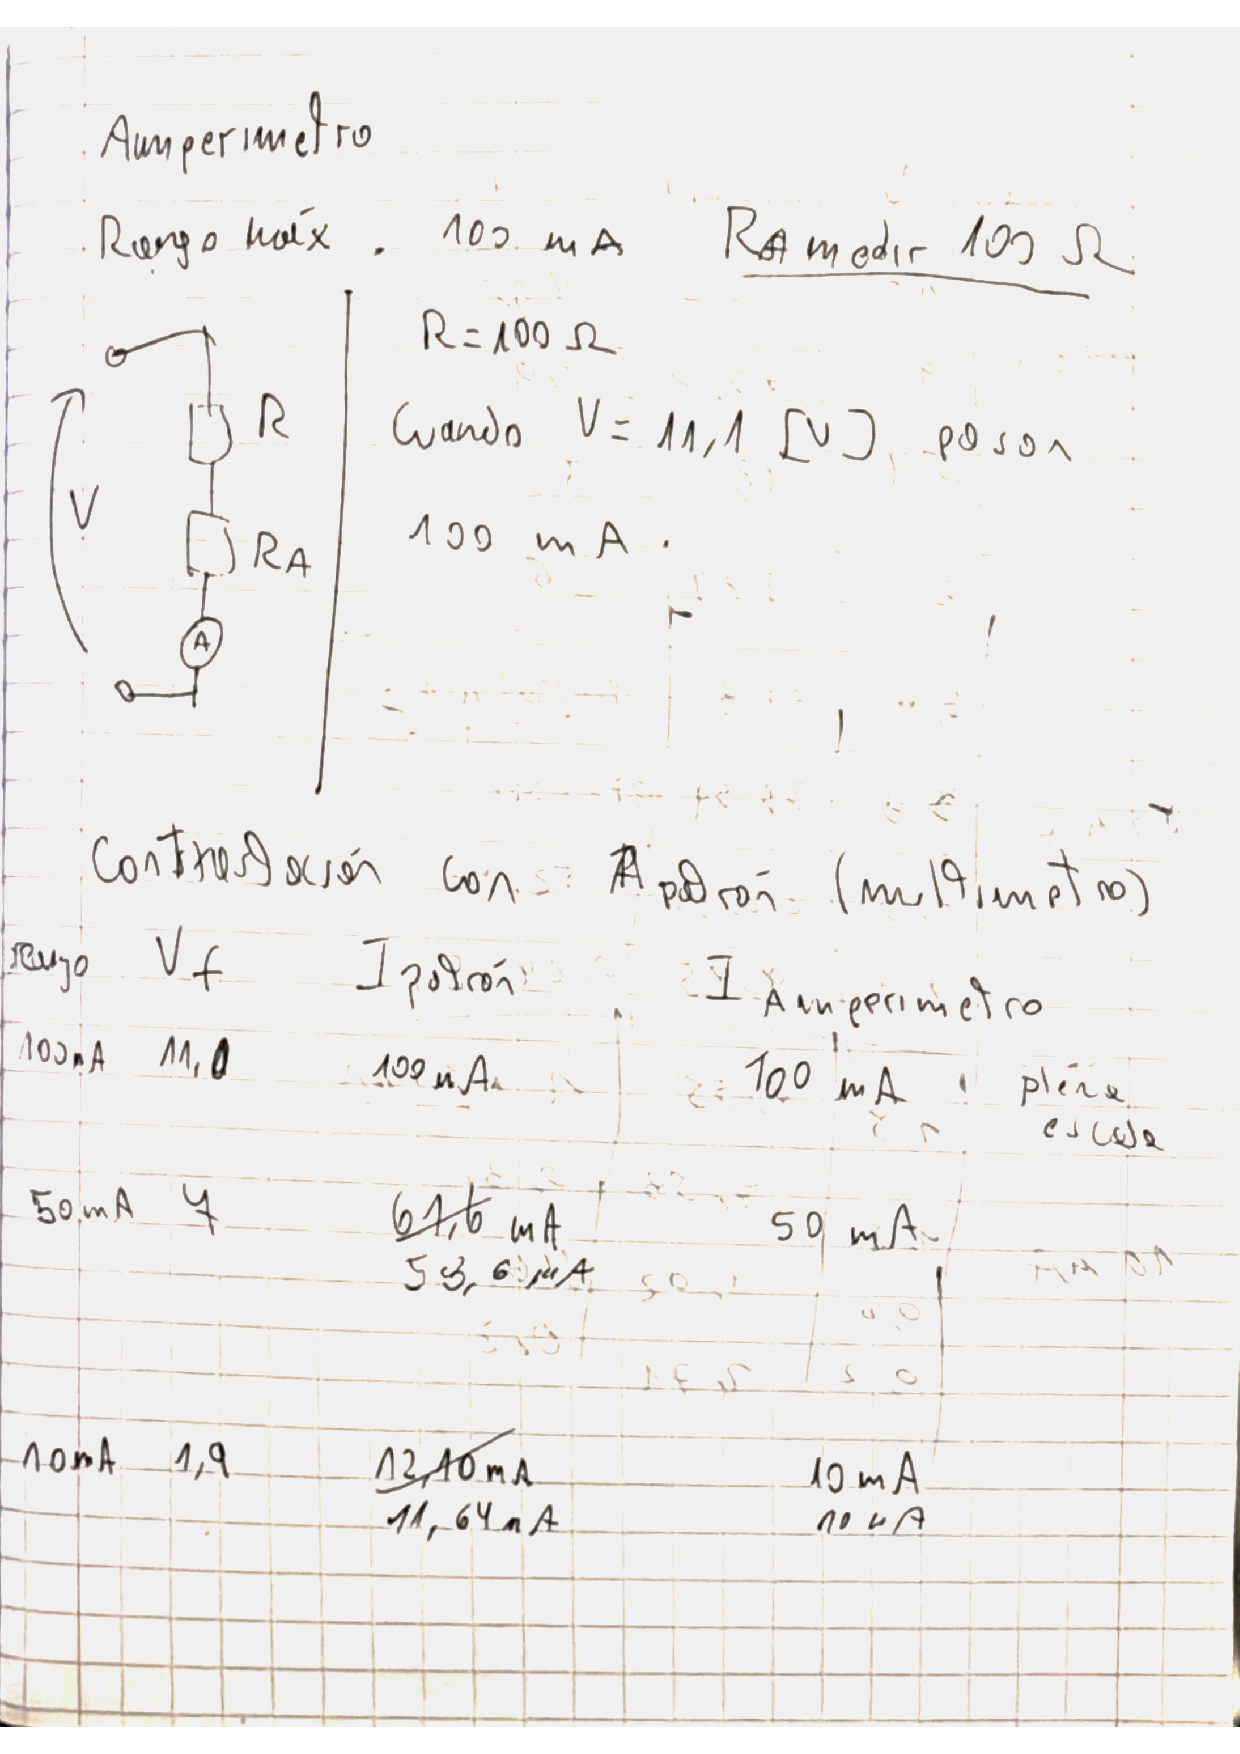
\includegraphics[width=0.8\linewidth]{recursos/10_1.pdf}
    \caption{Registro de los cálculos y contraste inicial del amperímetro analógico.
Se determinó la corriente total de 100 mA para el rango máximo con una resistencia limitadora de 100 $\Omega$.
Se observa el ajuste de la corriente del galvanómetro (Ig = 1 mA) y la corriente de prueba ($I_p$ = 100 mA) mediante la variación de $R_c$.
Además, se incluye la comparación con el amperímetro patrón (multímetro) para verificar la correspondencia de plena escala y los puntos intermedios de calibración.}
    \label{fig:placeholder}
\end{figure}


\begin{figure}[H]
    \centering
    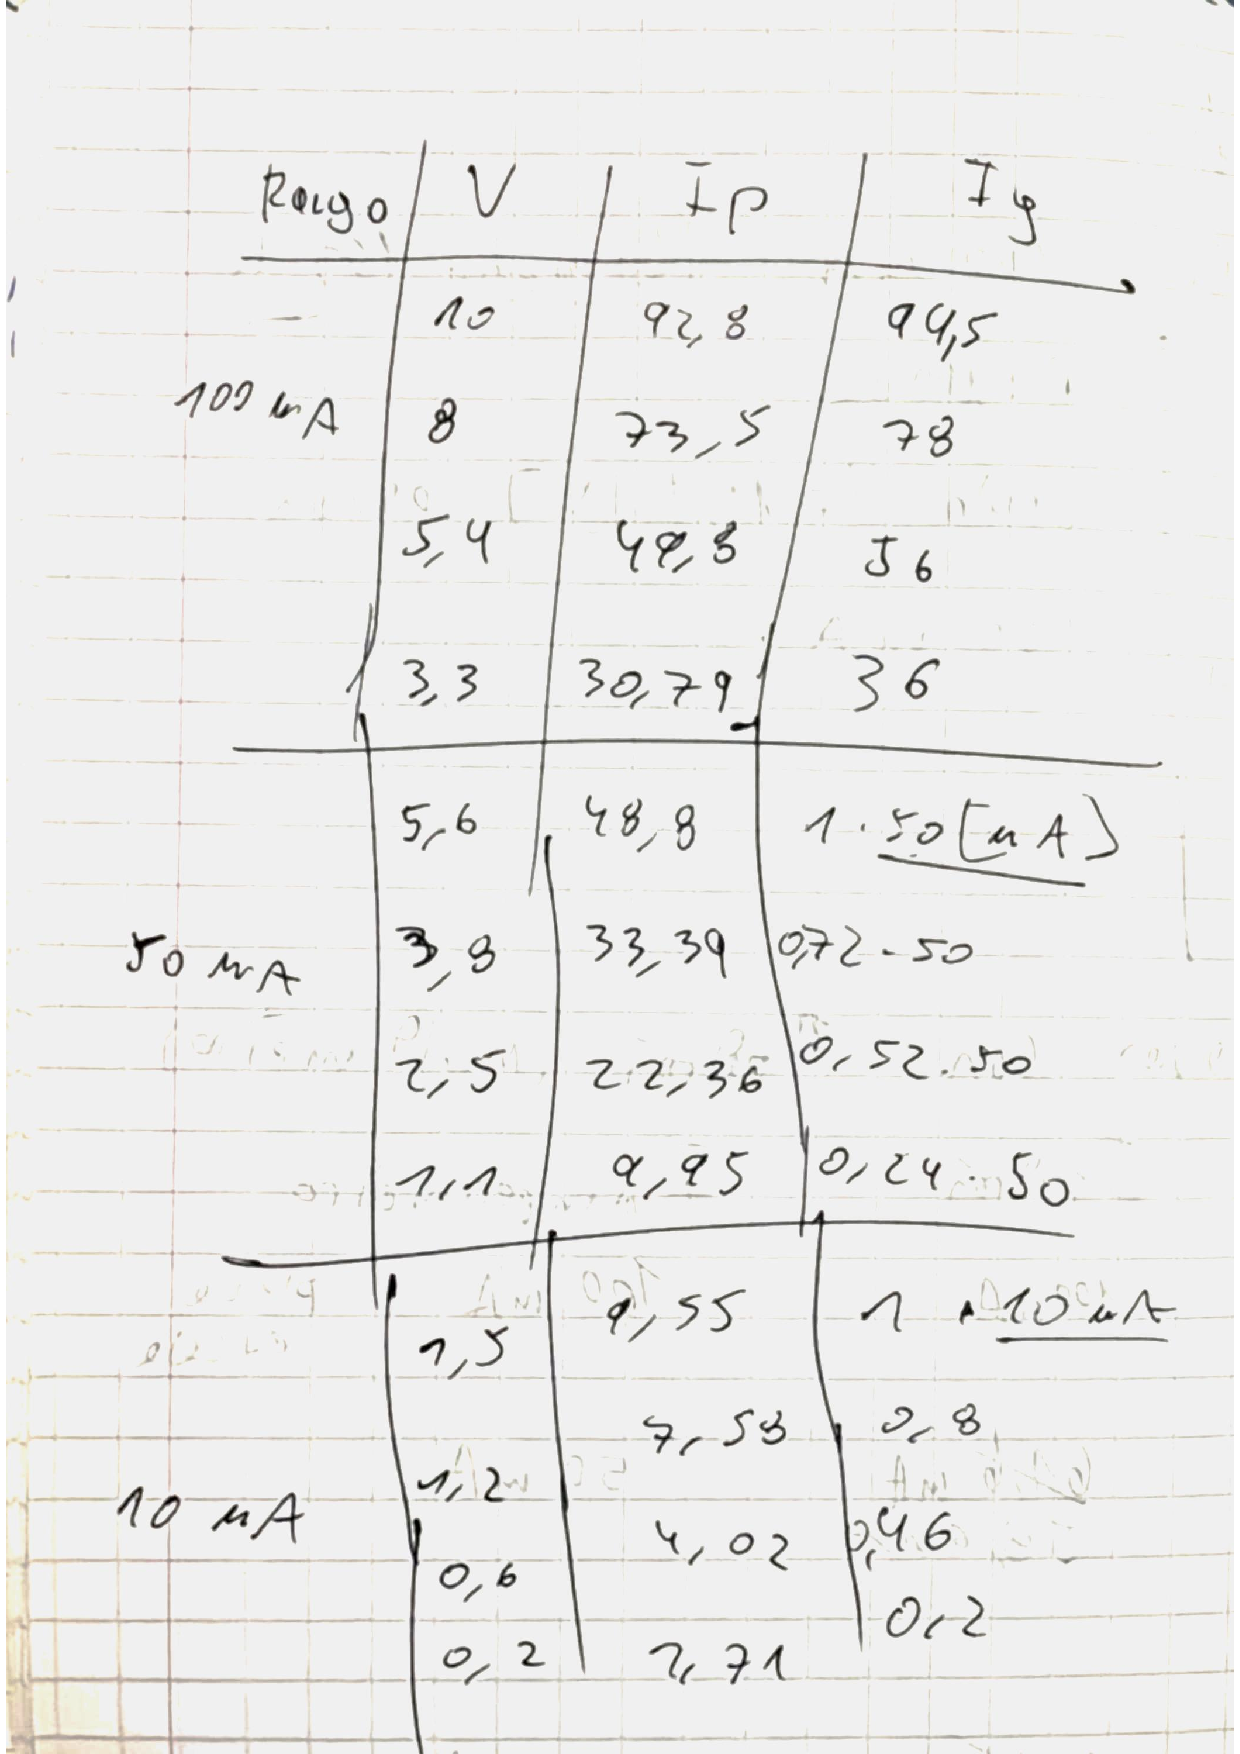
\includegraphics[width=0.8\linewidth]{recursos/10_2.pdf}
    \caption{Tabla de datos experimentales obtenidos en la verificación de la linealidad del amperímetro analógico.
Se registran los valores de tensión aplicada $V$, corriente patrón $I_p$ y corriente indicada por el galvanómetro $I_g$ en los tres rangos de medida: 100 mA, 50 mA y 10 mA.
Estos datos fueron utilizados para graficar la curva de linealidad y calcular el error porcentual de medición.}
    \label{fig:placeholder}
\end{figure}

\begin{figure}[H]
    \centering
    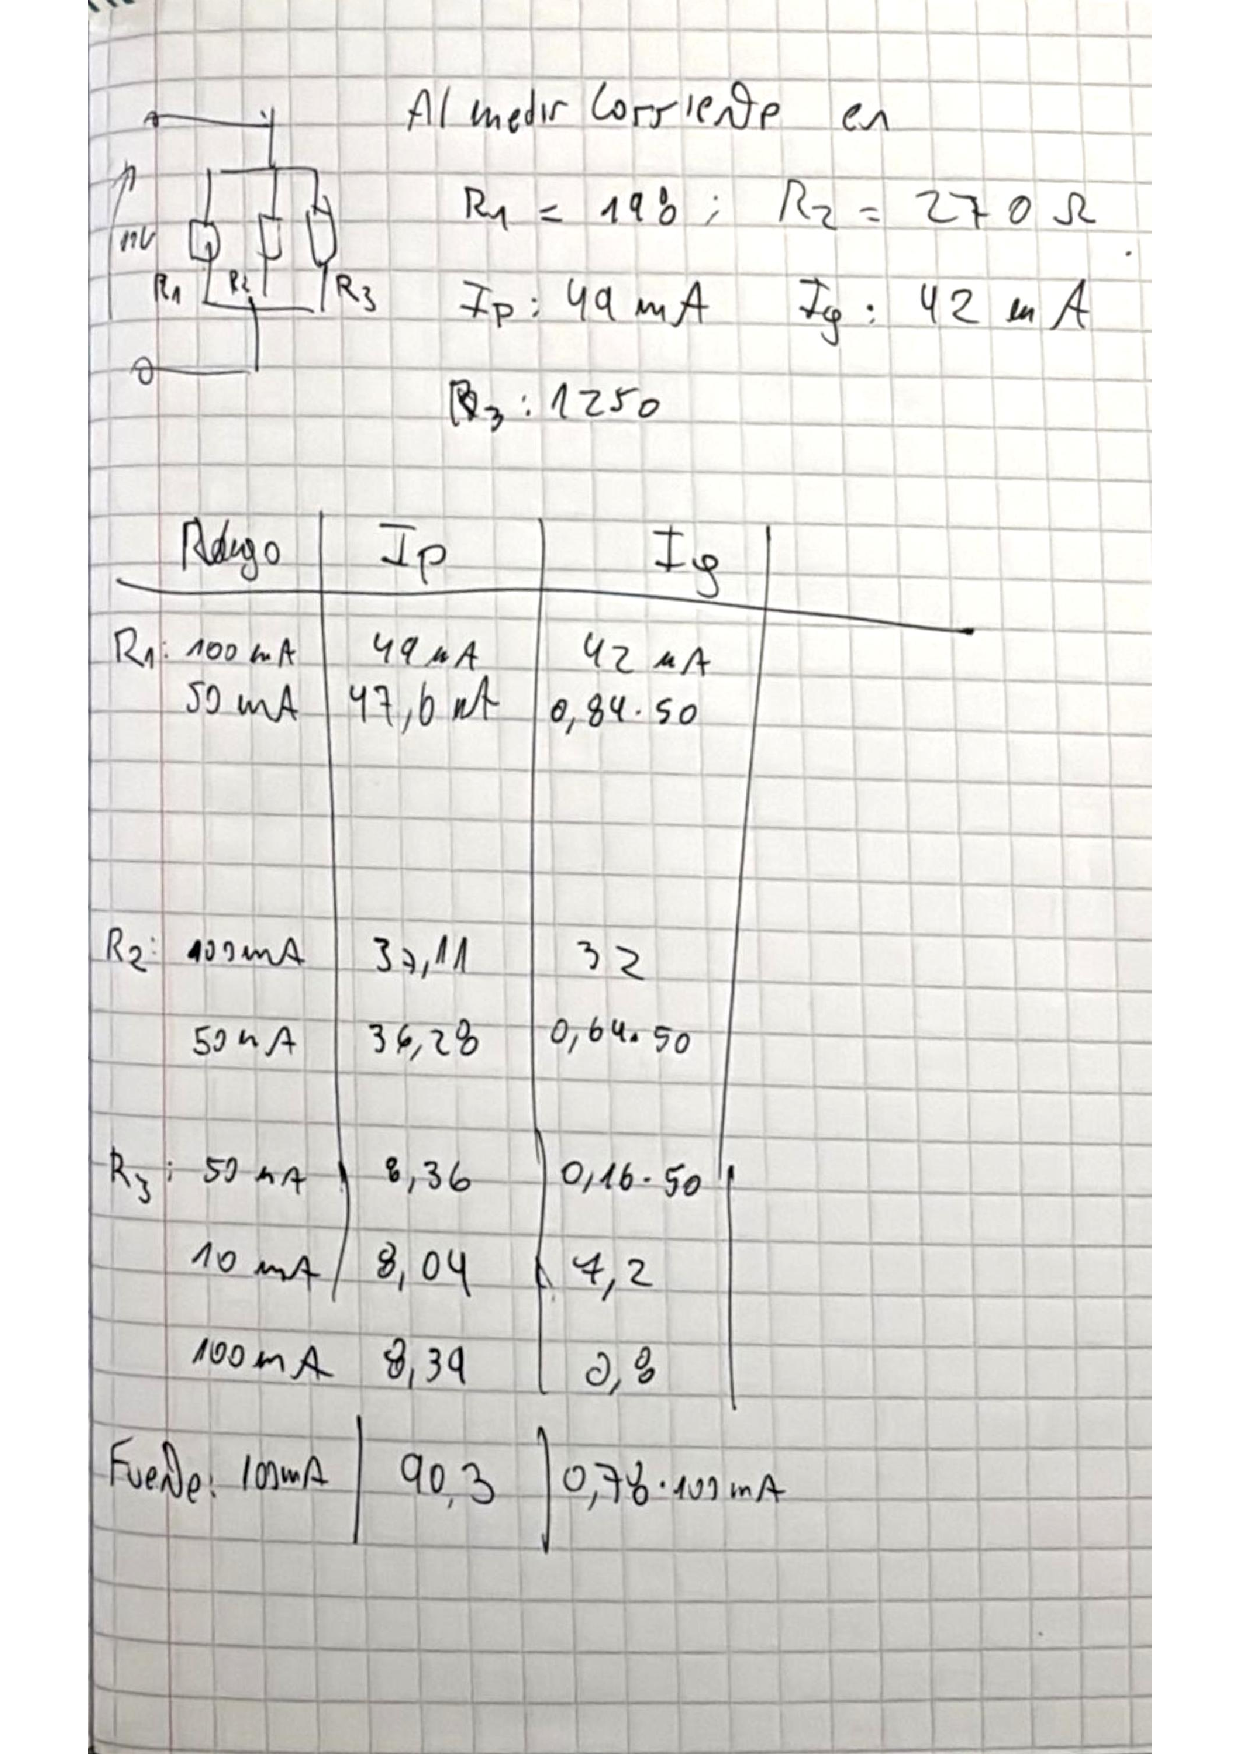
\includegraphics[width=0.8\linewidth]{recursos/10_3.pdf}
    \caption{Ensayo de medición de corrientes individuales y totales con resistores en paralelo.
Se utilizó una configuración con resistores de valores $R_1 = 198\, \Omega$, $R_2 = 270\ \Omega$, $R_3 = 125 \Omega$ aplicando una tensión de 10 $V_{cc}$.
Se compararon las corrientes medidas por el amperímetro $I_g$ con la corriente patrón $I_p$ en distintos rangos.
Este experimento permitió evaluar el error sistemático del instrumento y su comportamiento ante corrientes combinadas.}
    \label{fig:placeholder}
\end{figure}

\begin{figure}[H]
    \centering
    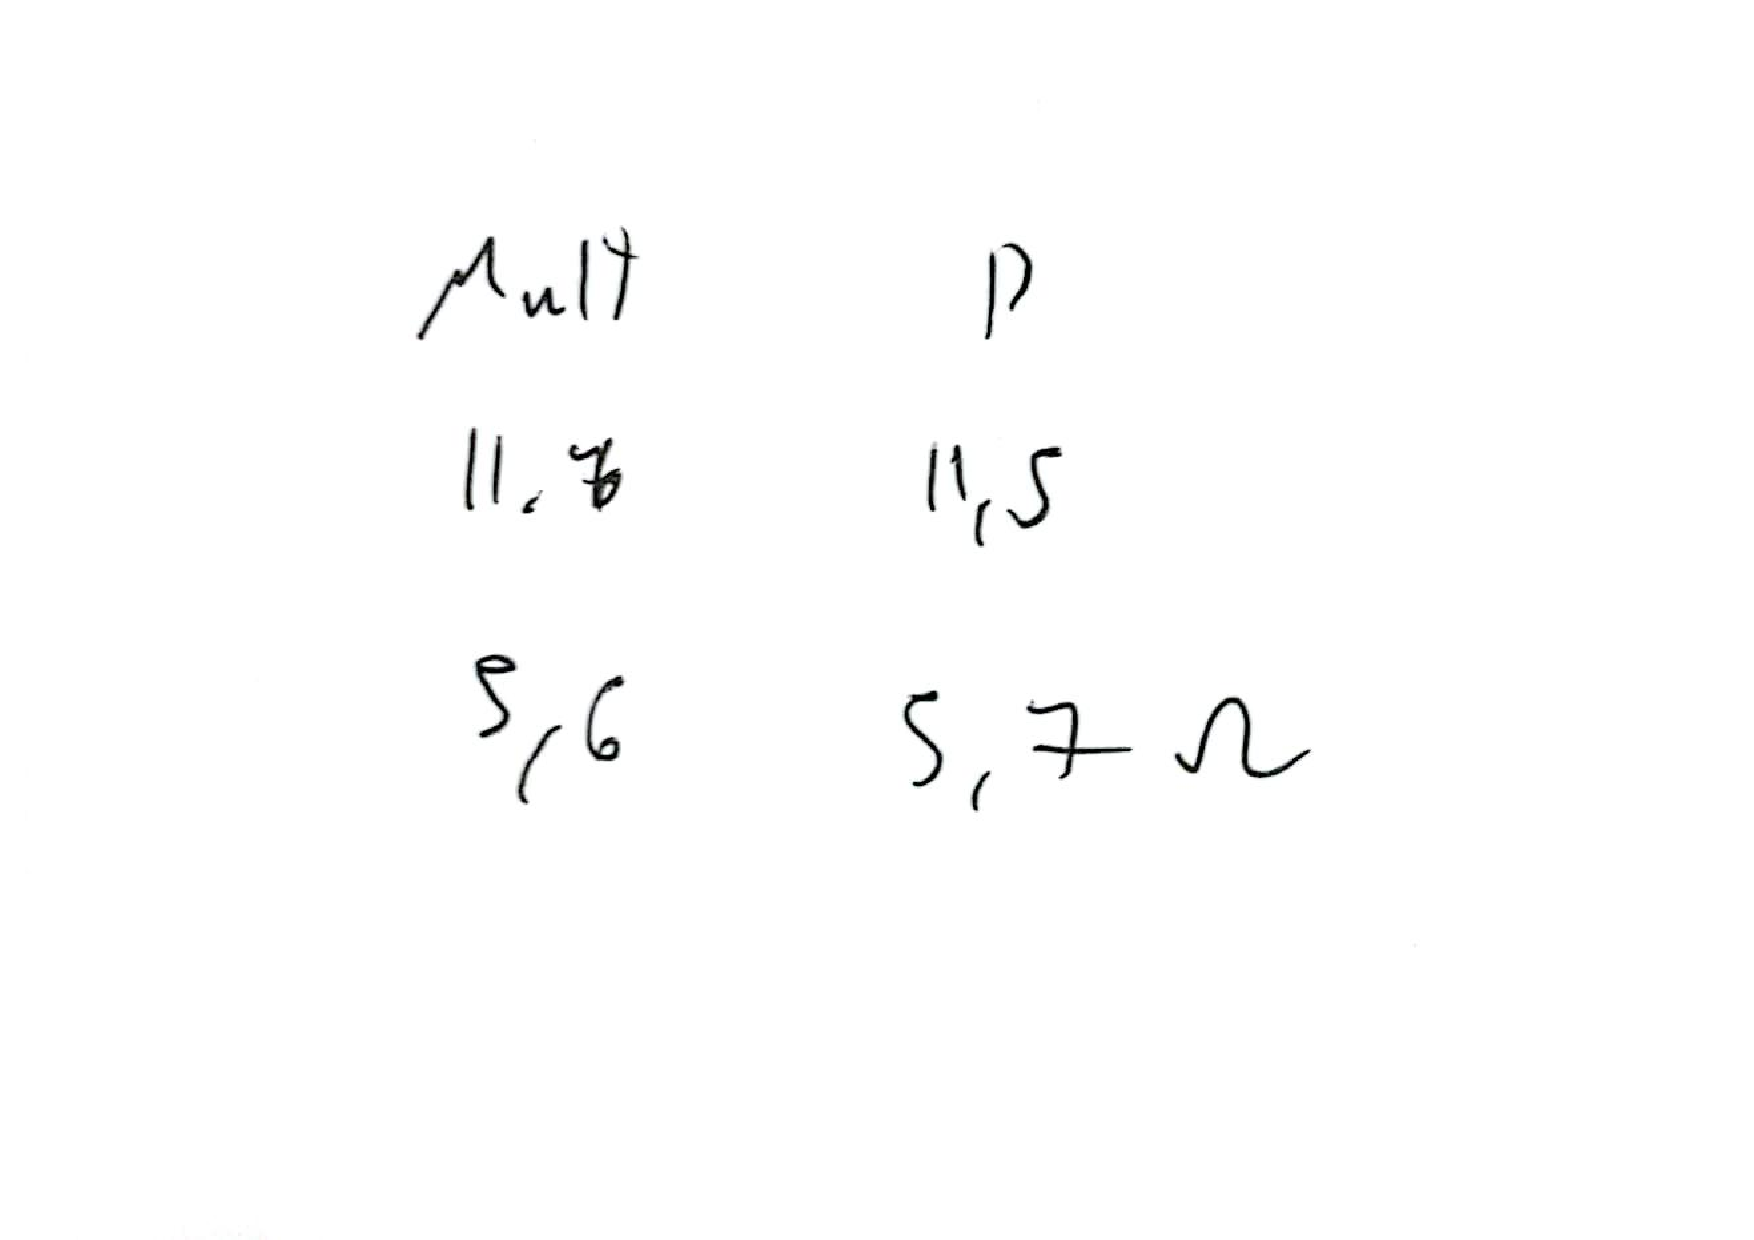
\includegraphics[width=0.75\linewidth]{recursos/10_4.pdf}
    \caption{En esta figura se presentan los resultados del contraste de las resistencias $R_{sh2}$ y $R_{sh3}$ utilizadas en el amperímetro analógico, medidas por dos métodos: con multímetro digital (columna “Mult”) y mediante el Puente de Kelvin (columna “P”).}
    \label{fig:placeholder}
\end{figure}



%\section{Referencias}
%\bibliographystyle{IEEEtran}
%\bibliography{sections/10referencias}

\end{document}